\documentclass[12pt]{article}

%**********************************************
%* Add additional packages as needed

\usepackage{url,amsmath,setspace,amssymb,graphicx}
\usepackage{listings}

\usepackage{tcolorbox}
\usepackage{tikz}
\usepackage{xcolor}


\usepackage{color}
\def\R{\color{red}}
\def\B{\color{blue}}

\usepackage{listings}
\usepackage{caption}


%**********************************************
%* Please replace this with your name and your AAU student number
\newcommand{\studentname}{Denis D'Ambrosi}
\newcommand{\studentnumber}{12245845}



%**********************************************
%* Some more or less useful stuff, add custom stuff as needed

\lstnewenvironment{myalgorithm}[1][] %defines the algorithm listing environment
{
   % \captionsetup{labelformat=algocaption,labelsep=colon}
    \lstset{ %this is the stype
        mathescape=true,
        frame=none,
        numbers=none,
        basicstyle=\normalsize,
        keywordstyle=\color{black}\bfseries\em,
        keywords={,input, output, return, datatype, function, in, if, else, foreach, while, begin, end, },
        numbers=left,
        xleftmargin=.04\textwidth,
        #1 % this is to add specific settings to an usage of this environment (for instance, the caption and referable label)
    }
}
{}


\newtcolorbox{alert}[1]{
colback=red!5!white, colframe=red!75!white,fonttitle=\bfseries, title = #1}

\newtcolorbox{commentbox}[1]{
colback=black!5!white, colframe=black!75!white,fonttitle=\bfseries, title = #1}



%**********************************************
%* Leave the page configuration as is
\setlength{\oddsidemargin}{.25in}
\setlength{\evensidemargin}{.25in}
\setlength{\textwidth}{6.25in}
\setlength{\topmargin}{-0.4in}
\setlength{\textheight}{8.5in}

\newcommand{\heading}[5]{
\renewcommand{\thepage}{#1-\arabic{page}}
\noindent
\begin{center}
	\framebox[\textwidth]{
	\begin{minipage}{0.9\textwidth} \onehalfspacing
	{\bf 622.755 -- \unitname} \hfill #2

	{\centering \Large #5

	}\medskip
	{#3 \hfill #4}
	\end{minipage}
}
\end{center}
}

\newcommand{\unitname}{Introduction to Cybersecurity}
\newcommand{\maxpages}{5}
\newcommand{\handout}[3]{\heading{#1}{#2}{\studentname}{\studentnumber}{#3}}

%**********************************************
%* The document starts here
\begin{document}
\handout{\maxpages}{Summer Term, 2022/23}{Project Write Up}

\section{Outline}

This report investigates the implementation of Yao's protocol within the field of financial data analysis from a social, legal and ethical perspective. The paper is structured as follows: section \ref{sec:yao} introduces the protocol itself and gives an overview of my implementation of the exchange, along with a relevant use case. Section \ref{sec:applications} investigates the deployment of Yao's protocol in some areas of financial data analysis, while section \ref{sec:sel} analyzes some of social, ethical and legal questions introduced with such technology. Finally, section \ref{sec:conclusions} briefly summarizes the contents of this report.

\section{Yao's protocol}\label{sec:yao}

Yao's protocol is a two-party secure computation protocol firstly introduced by Andrew Yao in 1982 \cite{Yao82} and then re-elaborated in 1986 \cite{Yao86} that enables two parties to jointly compute a function $f$ on their private inputs $x$ and $y$ without disclosing any information about those inputs to each other. 
The protocol relies on \textit{garbled circuits}, an algorithmic technique for encodes logical circuits so their inputs and outputs are hidden. To execute the protocol, one party (the garbler) encodes the circuit that computes the desired function $f$ along with its input $x$ and sends it to an evaluator who uses the encoded data to locally compute $f$ with $y$.
This \textit{Secure Multi Party Computation} (SMPC) exchange utilizes \textit{oblivious transfer}, a cryptographic exchange introduced by Rabin in an earlier paper \cite{OT} which allows one party to transfer only one of two values without disclosing which one was transferred and any information about the non-shared one. This prevents the garbler from learning anything about the evaluator's $y$.
Yao's protocol offers strong privacy assurances, as neither party gains any knowledge of the other's inputs or intermediate values computed during the protocol. This makes it ideal for applications where privacy is essential (see figure \ref{fig:applications}).

\begin{figure}[h]
    \centering
    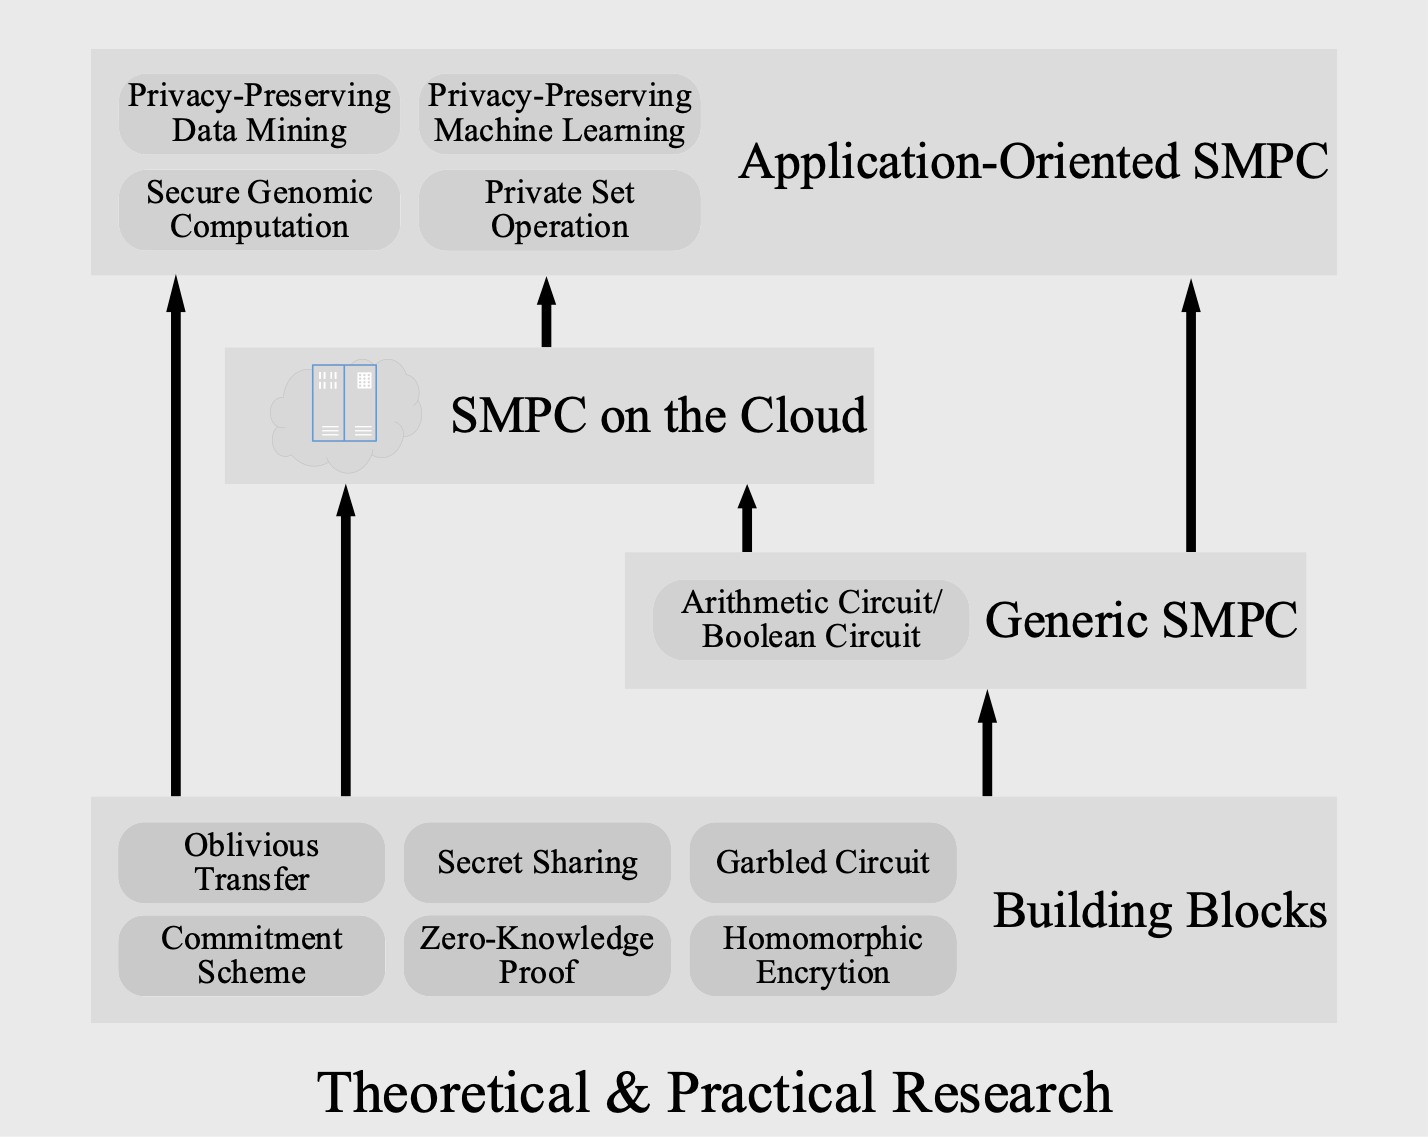
\includegraphics[width=0.6\textwidth]{practicalapplications.png}
    \caption{An overview of SMPC and its applications. Image taken from page 2 of \cite{Applications}.}\label{fig:applications}
\end{figure}

\section{Real-World Applications}\label{sec:applications}

In the implementation part of this project, I have implemented a garbled circuit that allows to securely compute a joint sum between two parties. In financial data analysis, this could be beneficial when organizations want to compile statistics together such as combined revenue of competing firms without disclosing individual revenues to each other. The protocol involves several cryptographic operations that enable these parties to compute the sum without sharing their inputs directly with one another.
Yao's protocol allows financial institutions to collaborate on data analysis tasks without exposing sensitive information \cite{Analysis}. This is especially helpful when complying with regulatory requirements or when parties are competitors who don't want to share proprietary data.

\subsection{Secure Financial Benchmarking}
One real-world application of Yao's protocol in financial analysis is secure financial benchmarking. This involves comparing an organization's performance against competitors, industry standards or historical data to identify areas for improvement and set performance targets. Unfortunately, sharing sensitive financial data with third-party benchmarking providers or competitors could pose privacy risks and potential misuse.
Yao's protocol-based secure benchmarking platform can give financial institutions the ability to compare their performance metrics without revealing actual data. A study by Brickell and Shmatikov \cite{Publishing} proposed an implementation of secure multi-party computation, using Yao's protocol, that allows banks to perform secure benchmarking for various financial metrics like loan default rates or operational costs without exposing sensitive information. This allows them to identify best practices and enhance their operations without risking sensitive information exposure.

\subsection{Secure Credit Scoring}

Another implementation of Yao's protocol in financial data analysis is secure credit scoring. Credit scoring plays an integral role in the lending process, helping financial institutions assess the risk associated with lending to a particular borrower. Unfortunately, credit scoring often necessitates sharing sensitive personal and financial data with the lender, raising privacy issues.

Researchers have proposed using Yao's protocol to create a secure credit scoring system that allows lenders to compute a credit score without directly accessing the borrower's private information \cite{Scoring}. In this arrangement, both parties jointly compute the score using Yao's protocol, with no knowledge of private data shared between them. This approach helps safeguard borrowers' privacy and alleviates concerns regarding misuse of personal data in credit scoring.

Furthermore, as proposed in \cite{ScoringMining}, it's possible to enhance secure credit scoring using privacy-preserving data mining \cite{Mining} to provide alternative input data sources in the credit assessment process, while still respecting privacy regulations.

\section{Ethical, Legal and Social Considerations}\label{sec:sel}

Yao's protocol can certainly offer financial data analysis many advantages, but there are several ethical, legal, and social concerns that must be taken into account.

\subsection{Ethical Considerations}

Yao's protocol can help protect sensitive data, but it is essential to guarantee that the secure computation process does not have unintended consequences such as discrimination or unfair treatment. For instance, in secure credit scoring, certain private data points could lead to biased scores or prevent some borrowers from accessing credit. Financial institutions must carefully evaluate both data inputs and algorithms used in secure computation to avoid potential ethical issues. In particular, these problems can occur in this field due to unbalanced data inputs and potential manipulation of the protocol's outcome. If these inputs are flawed, the resulting analysis could produce discriminatory results. For instance, if the input data is biased towards certain demographic groups, the resulting analysis could result in investment decisions that unfairly benefit those groups. Additionally, parties with greater resources or computing power could manipulate the protocol's outcome to their benefit, leading to unequal advantages for those in power. To address these concerns, it is essential to guarantee the data inputs used in the protocol are representative and unbiased, with appropriate safeguards in place to prevent manipulation of its outcome. Furthermore, one must take into account potential discriminatory outcomes when employing this protocol in financial data analysis, and take steps to mitigate those risks.

\subsection{Legal Considerations}

Yao's protocol must abide by relevant data protection and privacy regulations, such as the General Data Protection Regulation (GDPR) in the European Union or California Consumer Privacy Act (CCPA) in the United States: even though the garbled-circuit exchange is inherently privacy-oriented, it is imperative to always treat sensitive data confidentiality with extreme caution. These rules may impose specific requirements on how personal data should be handled even when encrypted to protect privacy and thus financial institutions must collaborate closely with legal counsel to guarantee adherence to all applicable laws and regulations. For instance, the deployment of an instance of Yao's protocol could lead to the sharing of sensitive personal information such as income, investment strategies and financial goals. If individuals do not give their consent or the data is inadequately protected, this data sharing could potentially violate said GDPR and CCPA regulations. To reduce privacy risks associated with the deployment of Yao's protocol in financial data analysis, any institution that implements it must ensure all personal data is anonymized and encrypted and appropriate consent and data security measures are in place.

\subsection{Social Considerations}

Yao's protocol and other secure computation techniques can contribute to a societal shift towards increased data privacy and security, yet it is essential to consider the potential impact on trust and transparency between parties involved. For example, using secure computation in financial benchmarking may raise concerns about data manipulation or cheating: any deviation from the agreed-upon inputs could lead to inaccurate or manipulated results. For instance, one party could provide false input data in order to influence the outcome of a computation to their advantage. Furthermore, an adversary with greater computing power or resources could, again, potentially exploit the protocol to their benefit. Financial institutions may thus need to establish appropriate governance structures, cryptographic verification techniques, secure computing infrastructure, and auditing procedures as well as collaborate with trusted third parties for integrity assurance in the secure computation process. By implementing these measures, one can guarantee the integrity of computation and protect against cheating by any party involved in its execution.

\section{Conclusion}\label{sec:conclusions}

After briefly introducing the dynamics of Yao's protocol, we have taken a look at some of its potential applications in financial data analysis that can allow organizations to collaborate on sensitive tasks without exposing private information. Examples such as secure financial benchmarking and credit scoring can give us a taste of its potential advantages; however, caution must still be exercised prior to implementation to ensure that deploying such secure exchanges does not introduce systematical discrimination, privacy violating mechanisms or opaqueness in the process.

\bibliographystyle{alpha}
\bibliography{references}
\end{document}



